\documentclass[twoside]{article}
\usepackage{fullpage}
\usepackage[pdftex]{graphicx}
\usepackage{wrapfig}
\usepackage{amsmath}
\usepackage{mathtools}
\usepackage{hyperref}
\usepackage{sectsty}
%\sectionfont{\fontsize{13}{15}\selectfont}
\usepackage{fixltx2e}
\usepackage{fancyhdr}
\usepackage{listings}
\usepackage{graphicx}
\pagestyle{fancy}
\fancyhead{}
\fancyfoot{}
\renewcommand{\headrulewidth}{0pt}
\fancyfoot[LO]{\emph{Cypes \(|\) James - CSI 370}}
\fancyfoot[R] {\thepage}
\newenvironment{code}{\fontfamily{lmtt}\selectfont}{}
\date{December 11, 2023}
\begin{document}
\title{Mathematical/Algorithmic Library}
\author{Jaden Cypes \(|\) Kathryn James\\CSI-370: Final Project}
\maketitle
\renewcommand{\labelitemi}{$\diamond$}


\noindent \textbf{INTRODUCTION}
\\Over the course of the semester, we have implemented various mathematical equations as well as basic instructions in assembly. Continuing on this theme, we created a Mathematical/Algorithmic Library that consists of matrix operations and sorting algorithms. The inspiration for this idea stemmed from everyone’s favorite classes at Champlain College: Linear Algebra and Data Structures \& Algorithms. With prior knowledge and understanding of these topics, we set out to implement these algorithms in assembly.\\


\noindent \textbf{REPOSITORY}
\\The Math/Algorithm Library repository can be found \href{https://github.com/katiepo456/math_algorithm_library}{here}.\\


\noindent \textbf{WHAT}
\\Our Mathematical/Algorithmic Library includes the following operations:
\begin{itemize}
\item \underline{Bubble Sort} is the simplest sorting algorithm that works by repeatedly swapping the adjacent elements if they are in the wrong order.
\item \underline{Selection Sort} is a simple and efficient sorting algorithm that works by repeatedly selecting the smallest (or largest) element from the unsorted portion of the list and moving it to the sorted portion of the list.
\item \underline{Insertion Sort} is a simple sorting algorithm where the array is virtually split into a sorted and an unsorted part; values from the unsorted part are picked and placed at the correct position in the sorted part.
\item \underline{Matrix Addition} is the operation of adding two matrices by adding the corresponding entries together.
\item \underline{Matrix Multiplication} is a binary operation that produces a matrix from two matrices.
\end{itemize}


\noindent \\ \textbf{WHY}
\\The challenge of implementing algorithms in low level languages such as assembly provides a good exercise and thought process into how algorithms at higher levels are translated into low level languages. With the intention of working on a software project, the creation of this library enabled us to draw connections to current and previous classes at Champlain College (Linear Algebra and Data Structures \& Algorithms). This project dives deeper into the assembly language by reworking algorithms and data types that we are already familiar with in a high-level language. Through research, review, and implementation, we broke complex operations - matrix addition/multiplication and sorting algorithms - down into smaller steps in order to rework these functions in MASM.\\


\noindent \textbf{HOW}
\\We sought to implement this project by using MASM in tandem with C++. The high-level language allows us to more easily provide console output so that the user can visually see the before and after of our mathematical/algorithmic operations. With the operations being defined in multiple .asm files, the project is dependent on the assembly language. We chose to do this program in x86\_64 assembly language due to its ability to pass parameters through registers to functions. This enabled better communication between our assembly and C++ code. The initial work was implemented in independent .asm files to ensure that the mathematical operation or sorting algorithm was working properly. Then we connected the functions to our C++ code along with creating some helper functions to provide console output to the user. Upon running the project, the C++ code calls various assembly functions in order to perform matrix addition, matrix multiplication, bubble sort, selection sort, and insertion sort.\\


\noindent \textbf{EXPLANATIONS}
\noindent \\ \textbf{I/O Details}
\\To display the resulting matrix in a readable format, we implemented the following function in a linked C++ file. After the matrix operation completed either its addition or multiplication, the following function would be called to print the matrix product or sum. Figure 1.1 shows the function needed to loop through the elements of the 2D array (matrix). It accounts for the number of rows and columns of the result and displays the resulting matrix accordingly. The function also receives a byte string as a parameter to use as a title for the result; Figures 2 and 3 show the declaration of the strings that would later be passed along to the C++ function as a second parameter for the title.
\begin{center} \begin{tabular}{c} \begin{lstlisting}
extern "C" void _printMatrix(int matrix[3][3], char* str) {
	int i, j, k, n = 3;

	cout << endl << str << endl;
	for (i = 0; i < n; ++i)
		for (j = 0; j < n; ++j)
		{
			cout << " " << matrix[i][j];
			if (j == n - 1)
				cout << endl;
		}
	return;
}
\end{lstlisting} \end{tabular} \end{center}
\begin{center}\textit{Figure 1.1: main.cpp}\end{center}
\begin{center} \begin{tabular}{c} \begin{lstlisting}
sum BYTE "Sum Matrix: ",0        ; title for the resulting matrix
\end{lstlisting} \end{tabular} \end{center}
\begin{center}\textit{Figure 2: matrixAddition.asm}\end{center}
\begin{center} \begin{tabular}{c} \begin{lstlisting}
mult BYTE "Product Matrix: ",0   ; title for the resulting matrix
\end{lstlisting} \end{tabular} \end{center}
\begin{center}\textit{Figure 3: matrixMultiplication.asm}\end{center}
For the sorting algorithms, the linked C++ file included a function to print out the arrays. After the completed sorts happen, the function shown in Figure 1.2 would be called at the bottom in the asm files to print to the console. The function would take the array and loop through each element, printing each to the console with a space in between. After the loop, a newline is printed so that the printed arrays do not mix.
\begin{center} \begin{tabular}{c} \begin{lstlisting}
extern "C" void _printNum(int arr[10]) {
	for (int i = 0; i < 10; i++) {
		cout << " " << arr[i];
	}
	cout << endl;
}
\end{lstlisting} \end{tabular} \end{center}
\begin{center}\textit{Figure 1.2: main.cpp}\end{center}
To create an array with a large undetermined size, filled with random numbers, it was decided to use a vector as it is flexible with adjusting its size. As well as creating a random\_device to make the random numbers. Using these two together made an ideal array to be sorted. 
\begin{center} \begin{tabular}{c} \begin{lstlisting}
	// create the random device engine
	random_device rd;
	mt19937 rng(rd());
	uniform_int_distribution<int> dist(1, 100);

	// create the array
	vector<int> vec;

	// declare size of vecotr and fill it with numbers
	const int vectorSize = 100;
	for (int i = 0; i < vectorSize; ++i) {
		int randNum = dist(rng);
		vec.push_back(randNum);
	}
\end{lstlisting} \end{tabular} \end{center}
\begin{center}\textit{Figure 1.3: main.cpp}\end{center}

\noindent \\ \textbf{Matrix Operations: Addition and Multiplication}
\\The two matrix operations that were implemented in this project include addition and multiplication. These functions were entirely written in assembly with the result then being passed to the C++ function \_printMatrix shown in Figure 1.1. Matrix addition can only be performed on matrices of the same size; each matrix must have the same number of rows and the same number of columns. For matrix multiplication, the number of columns on the first matrix must equal the number of rows on the second matrix. For the sake of simplicity, the implementation of these operations only works on square matrices of nxn size; the number of rows must match the number of columns.\\
\begin{itemize}
\item Matrix addition was implemented in assembly based on the C++ implementation from Figure 4. By using a nested for loop, the entries in the matrices are cycled through with each corresponding element in matrix A and matrix B being added together; the sum of the two elements is then stored in the corresponding location in the resulting matrix. The assembly implementation loads the two matrices into the rsi and rdi registers and performs matrix addition by looping through all of the elements, finding the sum of the corresponding elements between A and B, and storing the sum in its respective entry in the resulting matrix.
\end{itemize}
\begin{center} \begin{tabular}{c} \begin{lstlisting}
// Adding two matrices
    for(i = 0; i < n; ++i)
        for(j = 0; j < n; ++j)
            sum[i][j] = A[i][j] + B[i][j];
\end{lstlisting} \end{tabular} \end{center}
\begin{center}\textit{Figure 4: C++ Implementation of Matrix Addition}\end{center}
\begin{itemize}
\item Matrix multiplication was implemented in assembly based on the C++ implementation from Figure 5. By using a triple-nested for loop, the entries in the first row of matrix A are multiplied by the entries in the first column of matrix B. The dot product between each pairing is then added to the corresponding location in the resulting matrix. This process cycles through all rows/columns between both matrices. The assembly implementation computes the product of the two matrices that are loaded in the rsi and rdi registers through a triple-nested for loop.
\end{itemize}
\begin{center} \begin{tabular}{c} \begin{lstlisting}
// Multiplying matrix a and b and storing in array mult
    for(i = 0; i < n; ++i)
        for(j = 0; j < n; ++j)
            for(k = 0; k < n; ++k)
            {
                mult[i][j] += a[i][k] * b[k][j];
            }
\end{lstlisting} \end{tabular} \end{center}
\begin{center}\textit{Figure 5: C++ Implementation of Matrix Multiplication}\end{center}

\noindent \\ \textbf{Sorting Algorithms: Bubble, Selection, Insertion}
\\The sorting algorithms are entirely written in assembly with programmer-defined arrays. There is an included \_printNum C++ function to outprint the arrays. The goal was to use a much bigger vector array.\\
\begin{itemize}
\item Bubble Sort was implemented in assembly based on the C++ implementation shown in Figure 6. Using a nested for loop, both loops will use the length of the array to cycle through each element. The inner loop makes the comparisons while the outer loop runs the inner loop over and over until the array is sorted. The assembly implementation compares two elements next to each other from left to right. If the one on the left is bigger than the right, the elements will swap. If not, the comparison will skip to the next pair of elements. In the assembly implementation, the array address is loaded in rsi and the length into rcx. The rax and rbx registers are used in the comparison then rax is used to exchange the values in the array. 
\end{itemize}
\begin{center} \begin{tabular}{c} \begin{lstlisting}
    void bubbleSort(int array[], const int length) {
        int i, k;
        for (i = 0; i < length - 1; i++) { // loop through the array
            for (k = 0; k < length - i - 1; k++)  {
                if (array[k] > array[k + 1]) { // comparing in the second loop
                    swap(array[k], array[k + 1]); 
                }   
            }
        }
    }
\end{lstlisting} \end{tabular} \end{center}
\begin{center}\textit{Figure 6: C++ Implementation of Bubble Sort}\end{center}
\begin{itemize}
\item Selection Sort was implemented in assembly based on the C++ implementation shown in Figure 7. Using a nested for loop, the array length is used to cycle through and pick the smallest element and place it into a sorted portion of the array. Then the smallest element would be changed to the next element considered the smallest of the unsorted portion. In assembly, the array length and address would be loaded into rcx and rsi.  Other registers were used to keep track of the min element such as rdi or keep track of how many comparisons to make in rdx. 
\end{itemize}
\begin{center} \begin{tabular}{c} \begin{lstlisting}
    void selectionSort(int array[], const int length) {
        int i, k, minElement;
        for (i = 0; i < (length - 1); i++) {
            minElement = i; // to hold the smallest element at a time
            for (k = i + 1; k < length; k++){
                if (array[k] < array[minElement])
                    minElement = k; // changing the minElement
            }
            if (minElement != i)
                swap(array[minElement], array[i]);
        }
    }
\end{lstlisting} \end{tabular} \end{center}
\begin{center}\textit{Figure 7: C++ Implementation of Selection Sort}\end{center}
\begin{itemize}
\item Insertion Sort was implemented in assembly based on this C++ implementation. The sort is supposed to divide the array into two parts, sorted and unsorted. Therefore in this implementation, the idea of using registers as i and j, rax and rbx in this case. Then with rcx as the length of the array, and used as the counter for the loops, it could be used as the “key” during comparisons. The variable current represents this key, and in assembly, the rcx register would add rsi and rbx or rax to get to the current values being compared or swapped. 
\end{itemize}
\begin{center} \begin{tabular}{c} \begin{lstlisting}
void insertionSort(int array[], const int length) {
        int i, j;
        int current; //for comparing when shifting
        for (i = 1; i < length; i++) {
            current = array[i]; // continuing to move current along
           j = i - 1;
            while (j >= 0 && array[j] > current) { 
                array[k + 1] = array[k];
                j = j - 1;
            }
            array[j + 1] = current;
        }
    }
\end{lstlisting} \end{tabular} \end{center}
\begin{center}\textit{Figure 8: C++ Implementation of Insertion Sort}\end{center}

\noindent \\ \textbf{CHALLENGES AND SOLUTIONS}
\noindent \\ \textbf{File Confusion}
\begin{itemize}
\item Prior to starting the project, we were worried about how we would create multiple assembly files and link all of them to the same C++ main.cpp file. For the sake of organization, we thought that our project would be best suited to have an individual .asm file for each matrix operation or sorting algorithm; but we were unsure of how that would work. When actually starting the project, we learned that this was not a problem. So long as we included the prototype of the necessary C++ functions in the assembly file or vice versa, the overall program would continue to run smoothly by calling the various assembly functions from their respective .asm files.
\end{itemize}

\noindent \\ \textbf{Matrix Entry Access}
\begin{itemize}
\item Matrices function in C++ as 2D arrays; however, assembly treats multidimensional arrays as one long array. We would be unable to access the element of the matrix as [\textit{row}][\textit{column}], but rather as the $n^{\text{th}}$ element. This posed the challenge of finding the correct index number.
\end{itemize}
\centerline{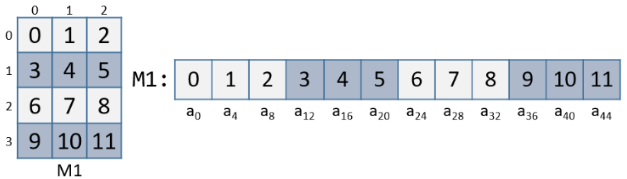
\includegraphics[scale=2]{images/matricesinmemory.png}}
\begin{center}\textit{Figure 9: Visual Representation of Matrices in Memory}\end{center}
\begin{itemize}
\item To access an element of the matrix as the $n^{\text{th}}$ element rather than [\textit{row}][\textit{column}], we did the following: multiply the entry location by the number of rows and then add the column number. This makes $a_{\text{21}}$ in the matrix become the $7^{\text{th}}$ element in the array.
\end{itemize}
\begin{itemize}
\item After finding the proper index using the aforementioned method, the element was accessed and then stored in a register using the following instruction: movsx rcx, WORD PTR[rsi][rax*4]. In this example, the matrix was stored in the rsi register and the index is stored in the rax register.
\end{itemize}

\noindent \\ \textbf{Size Memory Location}
\begin{itemize}
\item When implementing the matrix addition, it would occasionally send the program into an infinite loop. Upon debugging and searching for the problem, we found that the constant that we had declared for the size of the array was being overwritten in memory. This variable n was used in the comparisons for the for loops, so when it was overwritten the program continued endlessly. Figure 7 shows the progression of the size variable in memory until it gets overwritten as zero. To avoid this problem, we stored the variable in a register that would not be used elsewhere in the program (r10). This way we do not have to worry about the counter being overwritten in its memory location. Now when the comparison is performed at the end of the loop, the counter i or j is compared to the value of n now residing in the r10 register.
\end{itemize}
\centerline{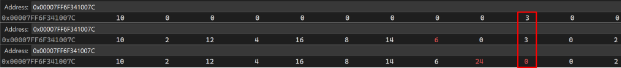
\includegraphics[scale=2]{images/countervalueoverwrite.png}}
\begin{center}\textit{Figure 10: Counter Value Overwrite}\end{center}

\noindent \\ \textbf{Back-to-Back Matrix Operations}
\begin{itemize}
\item In regards to the initial implementation of the matrix operations, we had one .asm file for the matrix operations and the C++ file. When trying to call the matrix operations back-to-back, i.e. \_matrixAdd and then \_matrixMultiplication, we were encountering errors where the defined values of a given matrix contained different values. We believe there was an issue with the way the memory was being allocated across all the matrices, but it was solved by creating an individual file for each matrix operation. Now the main function in the main.cpp file calls each function separately from their respective .asm files.
\end{itemize}

\noindent \\ \textbf{Programmer-Defined Arrays}
\begin{itemize}
\item Whether it is an issue with passing the array from C++ to MASM or receiving the array in assembly, we were unable to implement user-defined or randomly generated 2D arrays. This created the problem of only being able to use programmer-defined arrays found in the top of the .asm files: matrixMultiplication.asm and matrixAddition.asm. Rather than being able to test various randomly generated matrices, we were limited to using ones we had created ourselves as well as having to indicate the size of the square nxn matrix. Due to this ongoing issue, the matrix operations only work on square matrices to limit the amount of data entry on the programmer’s end.
\item The following code segment in Figure 8 shows the attempt at a function that will randomly generate and populate a 3x3 matrix. The matrix’s memory address is returned at the end of the function, but we were unable to actually access any of the values on the MASM side of the program. If future progress were made on this project, we would plan to implement this feature to fully access the elements in the assembly code.
\end{itemize}
\begin{center} \begin{tabular}{c} \begin{lstlisting}
extern "C" int** _getMatrix() {
	int N = 3, random;
	int** arr = new int* [N];
	srand(time(0));

	for (int i = 0; i < N; ++i) {
		arr[i] = new int[N];
		for (int j = 0; j < N; ++j) {
			random = 1 + (rand() % 10);
			arr[i][j] = random;
			cout << arr[i][j] << endl;
		}
	}
	return arr;
}
\end{lstlisting} \end{tabular} \end{center}
\begin{center}\textit{Figure 11: main.cpp}\end{center}

\noindent \\ \textbf{Swapping Elements of Arrays} 
\begin{itemize}
\item A recurring problem that ultimately proceeded to continue after finishing work on the project was the problem of swapping elements in an array. After getting the solution to accessing the value in an element of an array, the problem of exchanging or swapping the elements appeared. For some reason, the commands, xchg or even trying to swap manually using a temp variable did not manage to correctly exchange the values contained in the elements.  Unfortunately this was not solved at the end, and resulted in the sorts not being able to truly sort. 
\end{itemize}

\noindent \\ \textbf{Scope}
\begin{itemize}
\item Our worry going into this project dealt with understanding the scope of the project. The intent was to implement various sorting algorithms and other technical operations; however, we did not know to what extent we could implement in the given time frame. The plan was to implement the simple sorting algorithms (bubble, selection, and insertion) and the matrix operations (addition and multiplication). If time permitted, we hoped to progress into translating the higher-level sorting algorithms like merge sort and quicksort; however, we had to stop at the previously mentioned plan due to time constraints.
\end{itemize}


\noindent \\ \textbf{VISUALIZATIONS}
\\A sample of the console output after performing all the sorting algorithms and matrix operations.\\
\centerline{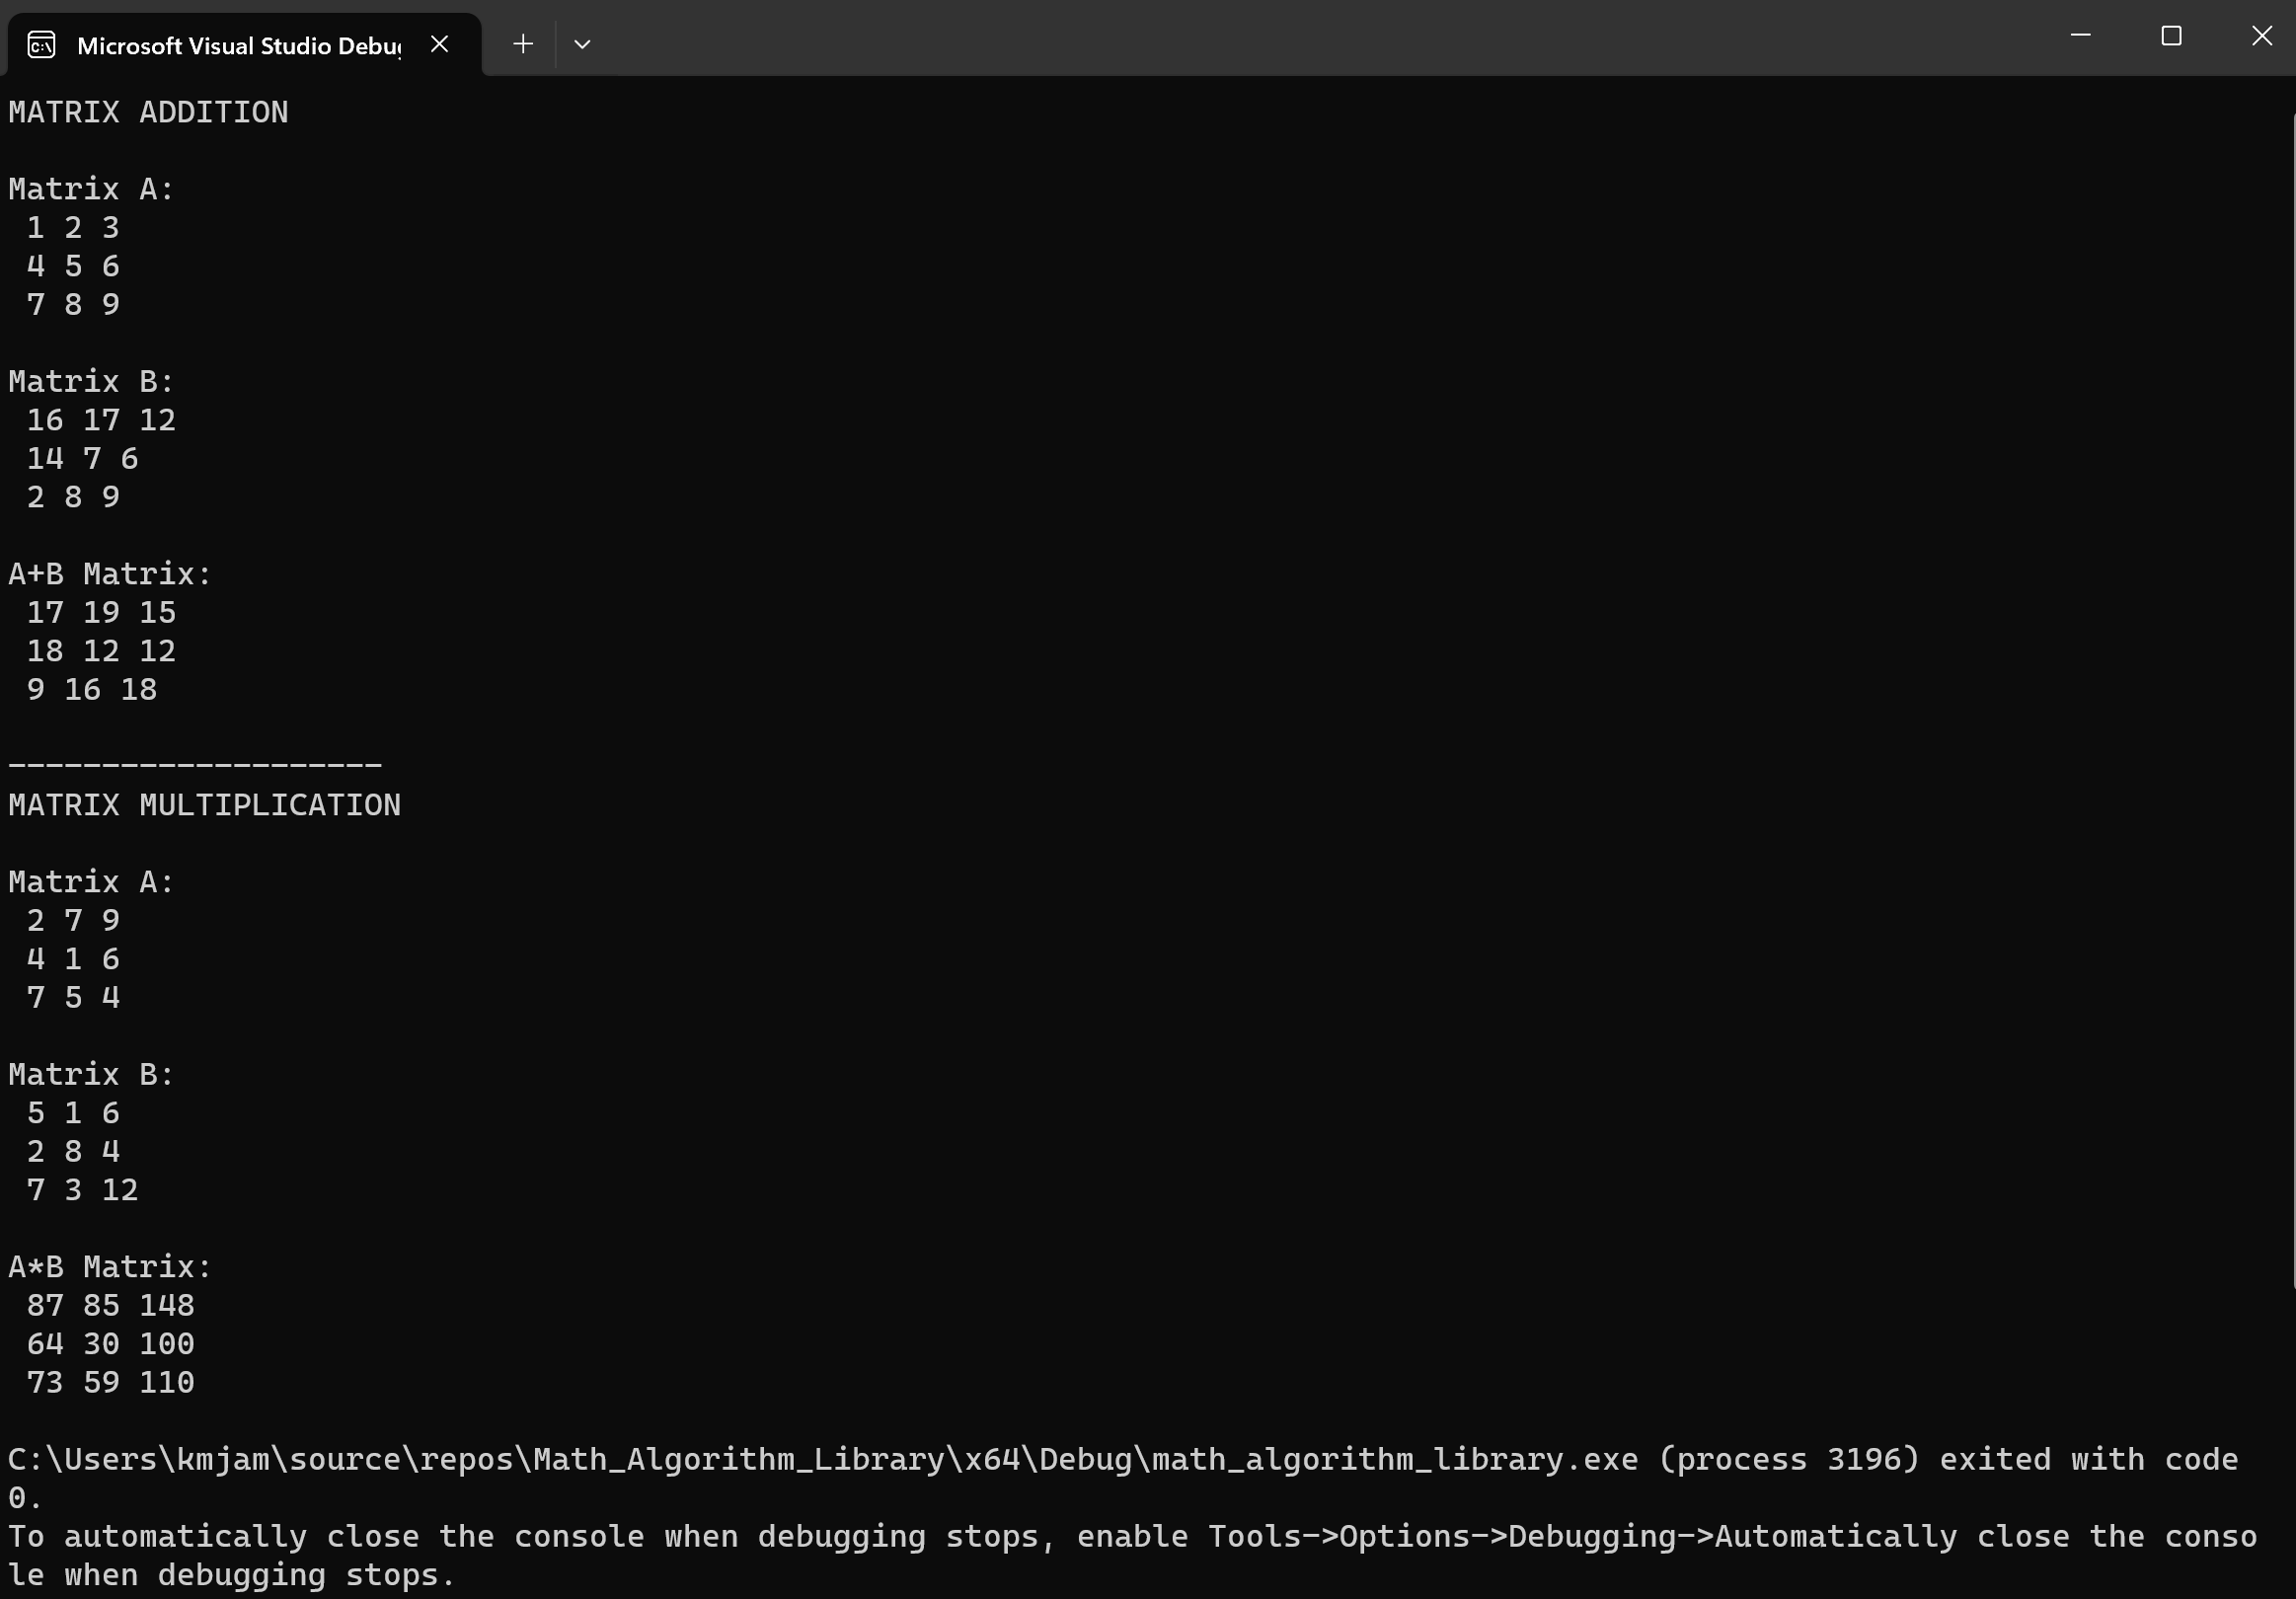
\includegraphics[scale=0.5]{images/matrixoperations.png}}
\begin{center}\textit{Figure 12: Console Output Window for Matrix Operations}\end{center}
\centerline{\includegraphics[scale=0.73]{Sortsoutput.png}}
\begin{center}\textit{Figure 13: Console Output Window for Sorting Algorithms}\end{center}


\newpage
\noindent \\ \textbf{SOURCES}
\begin{enumerate}
\item “C++ Program to Add Two Matrix Using Multi-Dimensional Arrays.” Programiz, \url{www.programiz.com/cpp-programming/examples/add-matrix}. Accessed 11 Dec. 2023.
\item “C++ Program to Multiply Two Matrix Using Multi-Dimensional Arrays.” Programiz, \url{www.programiz.com/cpp-programming/examples/matrix-multiplication}.
\item “Declaring and Defining an Array and Matrix in Assembly?” Stack Overflow, 2013, \url{https://stackoverflow.com/questions/17203771/declaring-and-defining-an-array-and-matrix-in-assembly}. Accessed 11 Dec. 2023.
\item “Exchange Instructions.” Exchange Instructions (IA-32 Assembly Language Reference Manual), Oracle Corp, 2010, \url{docs.oracle.com/cd/E19455-01/806-3773/6jct9o0bb/index.html.}
\item GeeksforGeeks. “Selection Sort - Data Structure and Algorithm Tutorials.” GeeksforGeeks, 31 Jan. 2014, \url{www.geeksforgeeks.org/selection-sort/}.
\item GeeksforGeeks. “Bubble Sort - Data Structure and Algorithm Tutorials.” GeeksforGeeks, 2 Feb. 2014, \url{www.geeksforgeeks.org/bubble-sort/}.
\item GeeksforGeeks. “Insertion Sort - Data Structure and Algorithm Tutorials.” GeeksforGeeks, 7 Mar. 2013, \url{www.geeksforgeeks.org/insertion-sort/}.
\item GrowCanadian. “MASM X86 Assembly - Need Help Adding to Array.” Reddit.com, 1 July 2019, \url{www.reddit.com/r/learnprogramming/comments/c7lvgj/masm_x86_assembly_need_help_adding_to_array/}. Accessed 11 Dec. 2023.
\item Hall, Brian R, and Kevin J Slonka. Assembly Programming and Computer Architecture for Software Engineers. Burlington Prospect Press, 2018.
\item “Matrix Addition.” Wikipedia, 17 Aug. 2021, \url{https://en.wikipedia.org/wiki/Matrix_addition}.
\item “Matrix Multiplication.” Wikipedia, 21 Oct. 2021, \url{https://en.wikipedia.org/wiki/Matrix_multiplication}.
\item “X86 MASM - Passing and Accessing a 2D Array.” Stack Overflow, 2017, \url{https://stackoverflow.com/questions/40962781/x86-masm-passing-and-accessing-a-2d-array}. Accessed 11 Dec. 2023.
\end{enumerate}


\end{document}